\section{Complexity Theory}\label{sec:3}

\subsection{Polynomial Time Reduction}\label{subsec:3.1}
In practice, we can only solve problems that have polynomial time algorithms, 
since they can scale to large problems when the corresponding constants 
are small. We have polynomial time algorithms for shortest path, 
primality testing, and linear programming; in contrast, it is unlikely 
that there are polynomial time algorithms for longest path, factoring, 
and integer programming. We would like to classify problems into two 
categories: those that can be solved in polynomial time, and those that 
cannot be. But the bad news is that a huge number of fundamental 
problems have defied classification for decades. 

We introduce the notion of {\bf polynomial time reduction}.

\begin{defn}{defn:3.1}
    We say that problem $X$ {\bf reduces} to problem $Y$ in polynomial time if 
    arbitrary instances of problem $X$ can be solved using a polynomial number 
    of standard computational steps, plus a polynomial number of calls to 
    an oracle that solves problem $Y$. We write $X \leq_P Y$ in this scenario. 
\end{defn}

This definition allows us to do a few things. 
\begin{enumerate}[(1)]
    \item {\bf Design algorithms.} If $X \leq_P Y$ and $Y$ can be solved in 
    polynomial time, then $X$ can also be solved in polynomial time. 
    \item {\bf Establish intractability.} If $X \leq_P Y$ and $X$ cannot be 
    solved in polynomial time, then $Y$ cannot be solved in polynomial time. 
    \item {\bf Establish equivalence.} If $X \leq_P Y$ and $Y \leq_P X$, then 
    we write $X \equiv_P Y$. In this case, $X$ can be solved in polynomial 
    time if and only if $Y$ can be. 
\end{enumerate}
The bottom line is that reductions allow us to classify problems according 
to relative difficulty. 

We give one example of a polynomial time reduction here, and refer to Chapter 
8 of Kleinberg and Tardos for many other examples. 

Recall that a {\bf literal} is a boolean variable or its negation, and a 
{\bf clause} is a disjunction of literals. A propositional formula $\Phi$ is 
in {\bf conjunctive normal form (CNF)} if it is a conjunction of clauses. 
For example, $\Phi = (x_1 \vee \overline{x_2}) \wedge (\overline{x_1} 
\vee x_3)$ is in CNF. 

The {\sc Sat} problem is as follows: given a propositional formula $\Phi$ in 
CNF, does it have a satisfying truth assignment? Then the {\sc $3$-Sat} problem 
is {\sc Sat} where each clause contains exactly $3$ literals, and each literal 
corresponds to a different variable. This has a key application in electronic 
design automation. One example of an instance of {\sc $3$-Sat} is 
\[ \Phi = (\overline{x_1} \vee x_2 \vee x_3) \wedge (x_1 \vee \overline{x_2} 
\vee x_3) \wedge (\overline{x_1} \vee x_2 \vee x_4), \] 
which has a satisfying truth assignment of $x_1 = {\sf T}$, $x_2 = {\sf T}$, 
$x_3 = {\sf F}$, and $x_4 = {\sf F}$. 

The {\sc Independent-Set} problem is as follows: given a graph $G = (V, E)$ 
and an integer $k$, is there a subset of $k$ (or more) vertices such that 
no two are adjacent? It turns out that {\sc $3$-Sat} can be reduced to 
{\sc Independent-Set}. 

\begin{theo}{theo:3.2}
    We have $\textsc{3-Sat} \leq_P \textsc{Independent-Set}$.
\end{theo}
\begin{pf}
    Let $\Phi$ be an instance of {\sc $3$-Sat}. We will construct an instance 
    $(G, k)$ of {\sc Independent-Set} that has an independent set of size $k$ 
    if and only if $\Phi$ is satisfiable. 

    Let $G$ be a graph which contains $3$ nodes for each clause, one for 
    each literal. Connect the $3$ literals in a clause in a triangle, 
    and connect every literal to its negations. 

    For example, with $k = 3$ and $\Phi = (\overline{x_1} \vee x_2 \vee x_3) 
    \wedge (x_1 \vee \overline{x_2} \vee x_3) \wedge (\overline{x_1} \vee 
    x_2 \vee x_4)$ as above, we can see that $G$ will be the following graph. 

    \begin{center}
        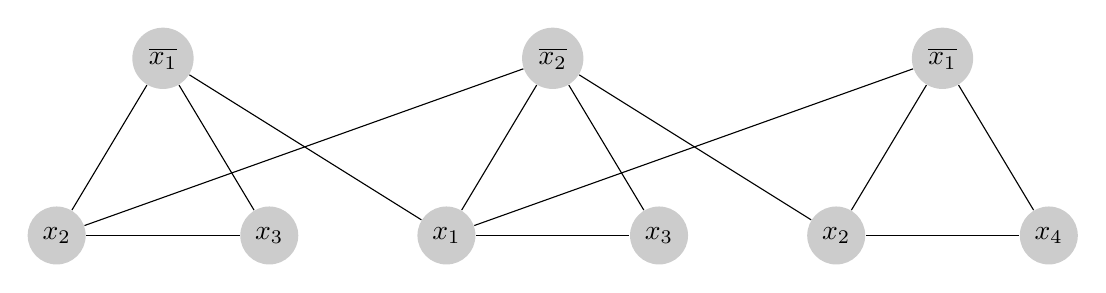
\begin{tikzpicture}  
          [scale=.9,auto=center,every node/.style={circle,fill=black!20}] % here, node/.style is the style pre-defined, that will be the default layout of all the nodes. You can also create different forms for different nodes.  
              
            \node (1) at (5, 2.5) {$\overline{x_1}$};  
            \node (2) at (3.5, 0) {$x_2$};  
            \node (3) at (6.5, 0) {$x_3$};

            \node (4) at (10.5, 2.5) {$\overline{x_2}$};
            \node (5) at (9, 0) {$x_1$};
            \node (6) at (12, 0) {$x_3$};

            \node (7) at (16, 2.5) {$\overline{x_1}$};
            \node (8) at (14.5, 0) {$x_2$};
            \node (9) at (17.5, 0) {$x_4$};
    
            \draw (1) -- (2);
            \draw (1) -- (3);
            \draw (2) -- (3);

            \draw (4) -- (5);
            \draw (4) -- (6);
            \draw (5) -- (6);

            \draw (7) -- (8);
            \draw (7) -- (9);
            \draw (8) -- (9);

            \draw (1) -- (5);
            \draw (5) -- (7);
            \draw (2) -- (4);
            \draw (4) -- (8);
            
        \end{tikzpicture} 
    \end{center}
    We claim that $\Phi$ is satisfiable if and only if $G$ contains 
    an independent set of size $k = |\Phi|$. 

    For the forward direction, consider any satisfying assignment for $\Phi$. 
    Then selecting one true literal from each clause (or triangle) will 
    give an independent set of size $k$. 

    Conversely, let $S$ be an independent set of size $k$. Then $S$ must 
    contain exactly one node in each triangle by construction. Set these 
    literals to ${\sf T}$ (and the remaining literals consistently). Then 
    all clauses in $\Phi$ are satisfied. This completes the proof. 
\end{pf}
